% =====================================================================
\section*{Question 2 -- Motion or Memory?}
\addcontentsline{toc}{section}{Question 2}

\noindent Hardware: MacBook Pro (2021), Apple M1 Pro, 32 GB (PyTorch 2.15.0, \texttt{mps} backend). Code: \texttt{Question2/} in the repository.

% ---------------------------------------------------------------------
\subsection*{1. Setup}

\begin{table}[H]\centering\small
\caption*{\textbf{Table 1.} Transform and window checks.}
\begin{adjustbox}{max width=\linewidth}\begin{tabular}{@{}llll@{}}
\toprule
 & Check & Expected & Yours\\
\midrule
(a) & $\max|M(M(x))-x|$ & 0 & 0 (\texttt{torch.equal}: True)\\
(b) & $\max|R^4(x)-x|$ & 0 & 0 (\texttt{torch.equal}: True)\\
(c) & $\max|MRM(x)-R^{-1}(x)|$ & 0 & 0 (\texttt{torch.equal}: True)\\
(d) & bright pixel of $M(p)$ & (7, 10, 43) & (7, 10, 43)\\
(e) & bright pixel of $R(p)$ & (7, 43, 10) & (7, 43, 10)\\
(f) & $1\times$ input / target & 1--5 / 6--10 & 1--5 / 6--10\\
(g) & $2\times$ input / target & 1, 3, 5, 7, 9 / 11, 13, 15, 17, 19 & 1, 3, 5, 7, 9 / 11, 13, 15, 17, 19\\
(h) & $3\times$ input / target & 1, 4, 7, 10, 13 / 16, 19 & 1, 4, 7, 10, 13 / 16, 19\\
\bottomrule
\end{tabular}\end{adjustbox}
\end{table}

\begin{figure}[H]\centering
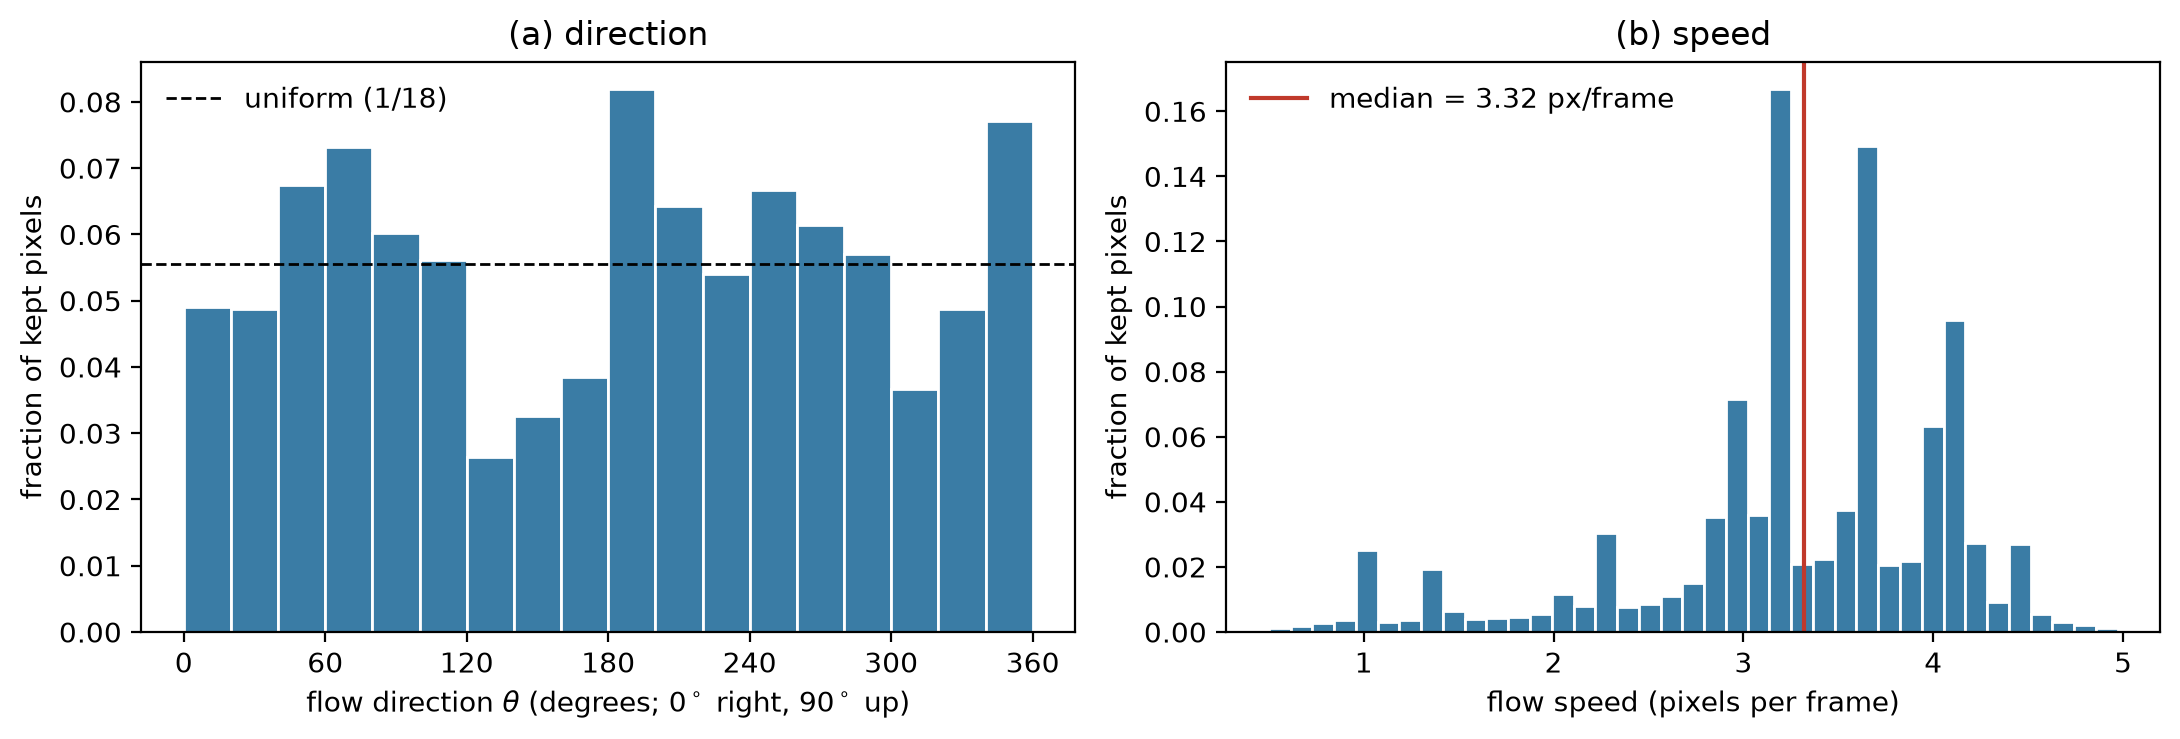
\includegraphics[width=\linewidth]{../Question2/figures/fig1_flow_stats.png}
\caption*{\textbf{Figure 1.} Farneback flow on the first 50 training videos (950 frame pairs, 103,050 pixels kept). (a) Direction, as a fraction of kept pixels; dashed line = uniform (1/18). (b) Speed; median 3.32 px/frame.}
\end{figure}

\paragraph{Q2.1.} Mirroring maps a direction $\theta$ to $180^\circ-\theta$ and a $90^\circ$ rotation maps it to $\theta+90^\circ$. Figure~1(a) has mass in every $20^\circ$ bin (0.026--0.082 against a uniform 0.056), and the unevenness has no clear axis, so it looks like sampling noise from 50 videos rather than a preferred direction. A mirrored or rotated histogram would look much the same, so mirrored and rotated \emph{motion} is already familiar. A typical speed is 3.3 px/frame (10--90\%: 2.1--4.1). At $2\times$ and $3\times$ the digits move about 6.6 and 10.0 px/frame, above almost every training speed, so faster motion is new. Flow is unreliable where digits overlap, but overlaps are a small share of the kept pixels and would add scattered errors in direction and speed rather than shift the whole histogram, so the answer would not change.

\paragraph{Q2.2.} Mirror and rotation keep the motion statistics (same speeds, directions already covered) but change the digits' appearance, rotation more than mirror. Speed-up keeps the appearance but changes the motion statistics. Each test therefore changes one factor, so a failure under mirror or rotation points to appearance, and a failure under speed-up points to motion.

% ---------------------------------------------------------------------
\subsection*{2. Baseline: ConvLSTM}

\paragraph{Q2.3.} One cell of the folded $16\times16$ grid is 4 original pixels. A $3\times3$ convolution moves information by at most one cell (4 px); the $1\times1$ output convolution and pixel (un)shuffle move nothing, and the cell-state update is element-wise. Within one step $\tau$, the longest path is $u_\tau$ (or $h^{(1)}_{\tau-1}$) $\to$ layer-1 convolution $\to h^{(1)}_\tau \to$ layer-2 convolution $\to h^{(2)}_\tau \to \hat x_{\tau+1}$: two $3\times3$ convolutions, so 2 cells $=$ \textbf{8 px per time step}. The path from $h^{(2)}_{\tau-1}$ crosses only the layer-2 convolution (4 px).

\begin{table}[H]\centering\small
\caption*{\textbf{Table 2.} Test error at $1\times$ ($t=1$), mean (seed 0, seed 1).}
\begin{adjustbox}{max width=\linewidth}\begin{tabular}{@{}lccccccr@{}}
\toprule
 & MSE$_1$ & MSE$_2$ & MSE$_3$ & MSE$_4$ & MSE$_5$ & $E^{(5)}$ & Params\\
\midrule
A & \makecell{0.0172\\(0.0176, 0.0167)} & \makecell{0.0205\\(0.0210, 0.0200)} & \makecell{0.0228\\(0.0233, 0.0222)} & \makecell{0.0244\\(0.0250, 0.0238)} & \makecell{0.0260\\(0.0266, 0.0255)} & \makecell{0.0222\\(0.0227, 0.0216)} & 480,784\\
Blank & 0.0426 & 0.0426 & 0.0426 & 0.0425 & 0.0425 & 0.0426 & 0\\
Copy-last & 0.0492 & 0.0604 & 0.0669 & 0.0708 & 0.0732 & 0.0641 & 0\\
\bottomrule
\end{tabular}\end{adjustbox}
\end{table}

\begin{figure}[H]\centering
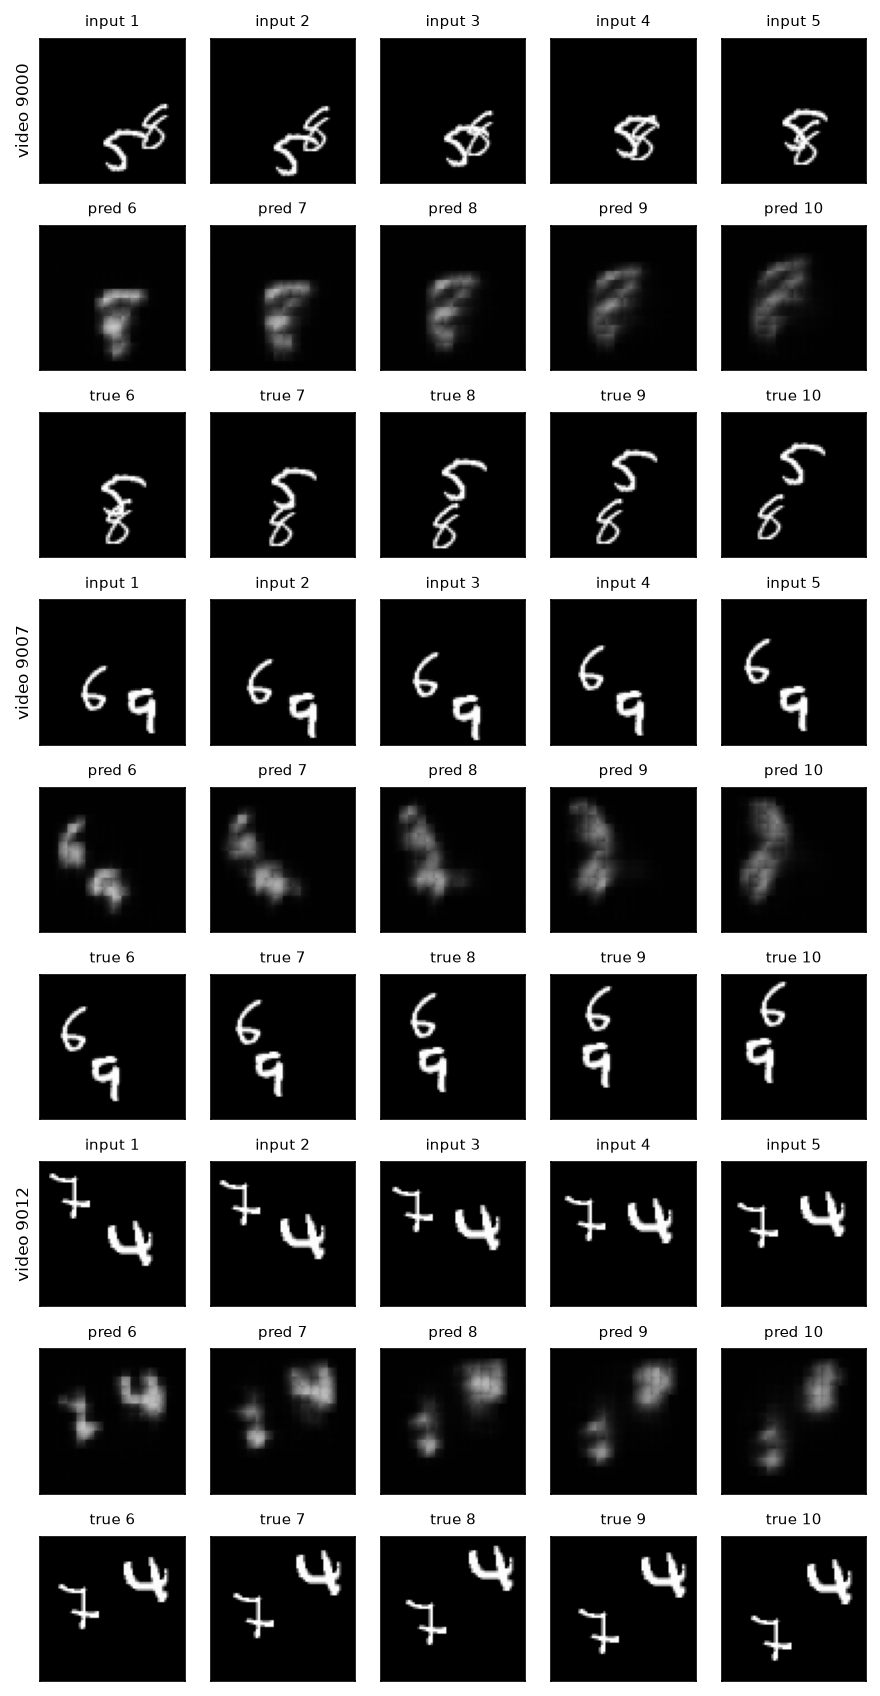
\includegraphics[width=0.62\linewidth]{../Question2/figures/fig2_A_predictions.png}
\caption*{\textbf{Figure 2.} Model A (seed 0) on three test videos: input frames 1--5, prediction and ground truth for frames 6--10. In video 9000 a 5 and an 8 overlap in the input and separate in the target.}
\end{figure}

\paragraph{Q2.4.} Model A beats both references at every horizon: its $E^{(5)}=0.0222$ is about half of Blank (0.0426) and a third of Copy-last (0.0641), so it does more than reproduce the last frame. Its error grows steadily, from 0.0172 at $h=1$ to 0.0260 at $h=5$ (about $1.5\times$), because each prediction is fed back as the next input and errors accumulate. Blank stays flat and Copy-last grows faster (0.0492 to 0.0732). Figure 2 shows why the error stays well above zero: positions are tracked roughly, but the digits blur within two or three steps and lose their identity. When digits overlap (video 9000), the model predicts one merged blob that drifts as a whole; it never separates the 5 and the 8, which in the true future move apart in opposite directions.

\paragraph{Q2.5 (written before testing).} Reach of model A (Q2.3): about 8 px per time step. Typical training speed (Figure 1): 3.3 px/frame (10--90\%: 2.1--4.1). \textbf{Mirror:} passes, mostly. Mirrored motion is already common in training (Figure 1a covers all directions), so the motion should carry over. Mirrored digits look unfamiliar, so expect some blurring of digit shape, and $C_M$ small but not zero. \textbf{Rotation:} passes the motion part but worse than mirror. Rotated motion is also familiar, but a sideways digit is less like any training digit than a mirrored one, so $C_R > C_M$. \textbf{Speed:} $2\times$ ($\approx$ 6.6 px/frame) is inside the 8 px reach but above every training speed, so predictions degrade but still follow the digits. $3\times$ ($\approx$ 10 px/frame) is beyond the reach, so the model breaks down there: digits stall or fade near their last input position.

% ---------------------------------------------------------------------
\subsection*{3. Testing the Baseline}

\begin{table}[H]\centering\small
\caption*{\textbf{Table 3.} Consistency gaps and transformed errors at $1\times$, mean (seed 0, seed 1).}
\begin{adjustbox}{max width=\linewidth}\begin{tabular}{@{}lccccc@{}}
\toprule
 & $E^{(5)}$ & $C_M$ & $E_M$ & $C_R$ & $E_R$\\
\midrule
A & 0.0222 (0.0227, 0.0216) & 0.00176 (0.00158, 0.00195) & 0.0228 (0.0233, 0.0223) & 0.00289 (0.00260, 0.00318) & 0.0239 (0.0242, 0.0236)\\
Blank & 0.0426 & 0 & 0.0426 & 0 & 0.0426\\
Copy-last & 0.0641 & 0 & 0.0641 & 0 & 0.0641\\
\bottomrule
\end{tabular}\end{adjustbox}
\end{table}

\begin{figure}[H]\centering
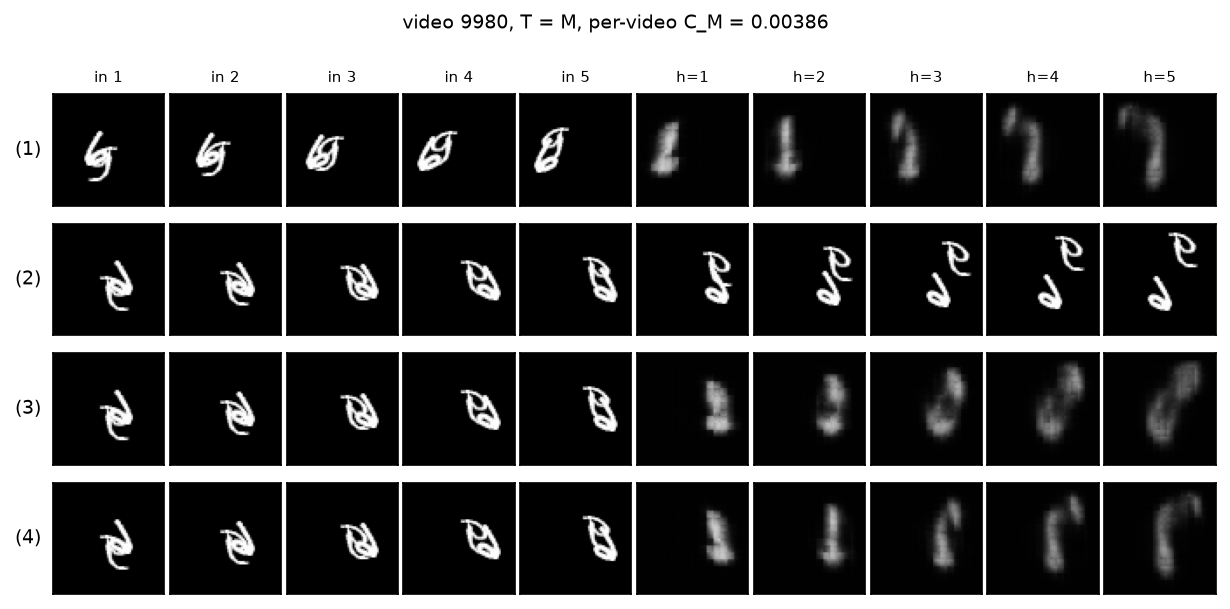
\includegraphics[width=0.49\linewidth]{../Question2/figures/fig3_A_M1_video9980.png}\hfill
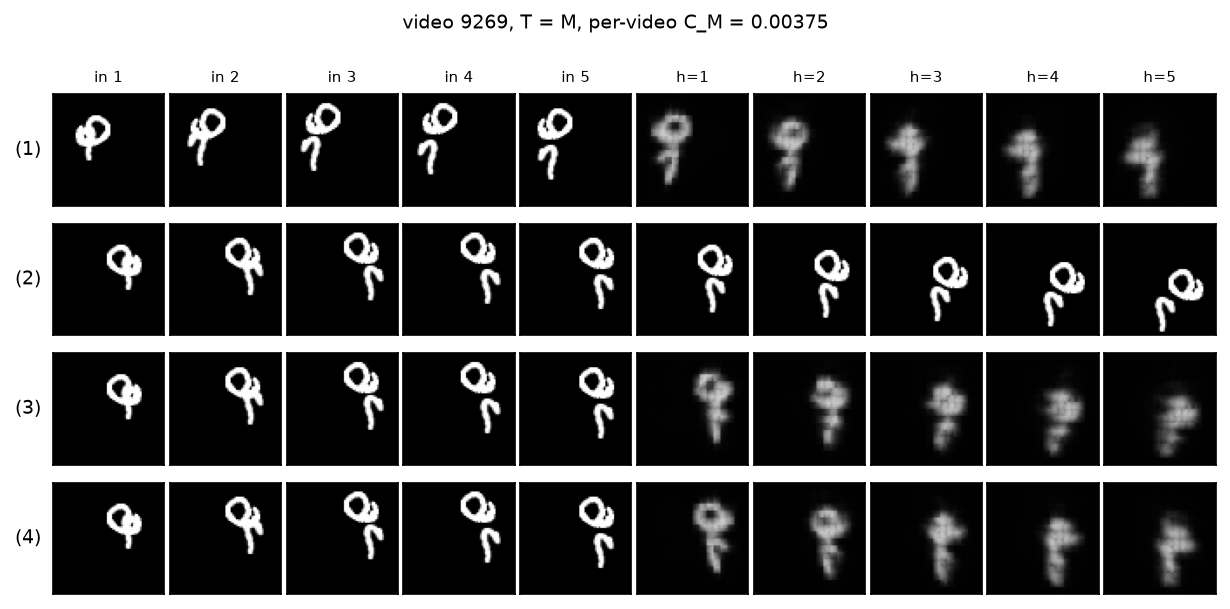
\includegraphics[width=0.49\linewidth]{../Question2/figures/fig3_A_M2_video9269.png}\\[4pt]
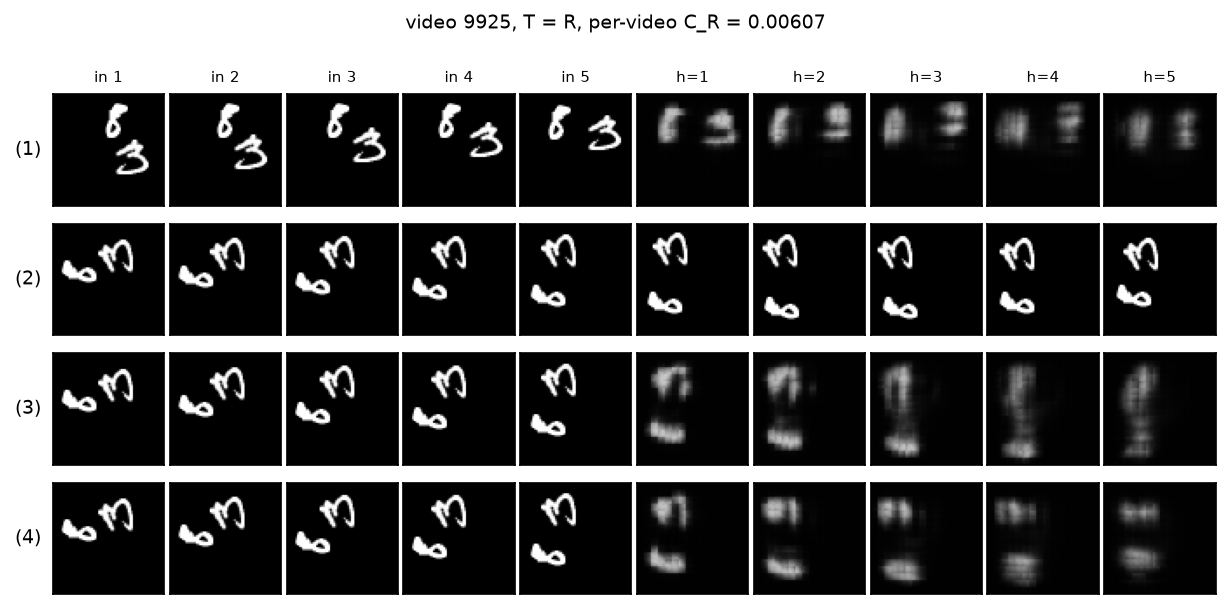
\includegraphics[width=0.49\linewidth]{../Question2/figures/fig3_A_R1_video9925.png}\hfill
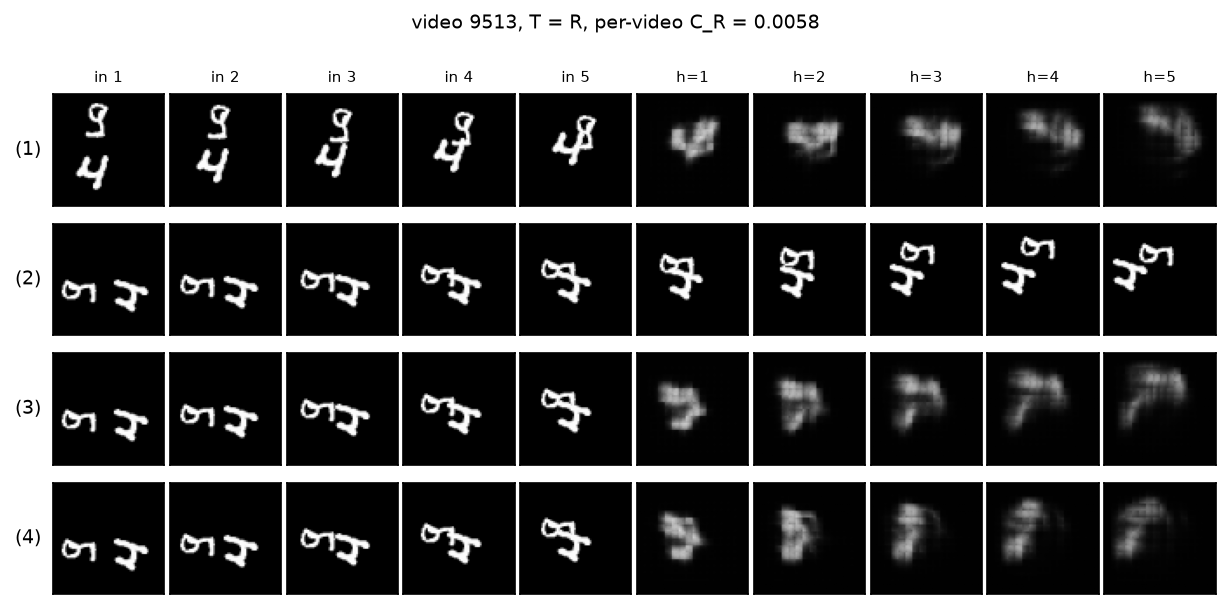
\includegraphics[width=0.49\linewidth]{../Question2/figures/fig3_A_R2_video9513.png}
\caption*{\textbf{Figure 3.} Test videos with the largest per-video $C_M$ (top) and $C_R$ (bottom), seed-0 model A. Columns 1--5: input; 6--10: horizons 1--5. Rows: (1) $X\,|\,f(X)$, (2) $T(X)\,|\,T(Y)$, (3) $T(X)\,|\,f(T(X))$, (4) $T(X)\,|\,T(f(X))$. GIFs: \texttt{Question2/gifs/fig3\_A\_M\_video9980.gif}, \texttt{fig3\_A\_M\_video9269.gif}, \texttt{fig3\_A\_R\_video9925.gif}, \texttt{fig3\_A\_R\_video9513.gif}.}
\end{figure}

\begin{figure}[H]\centering
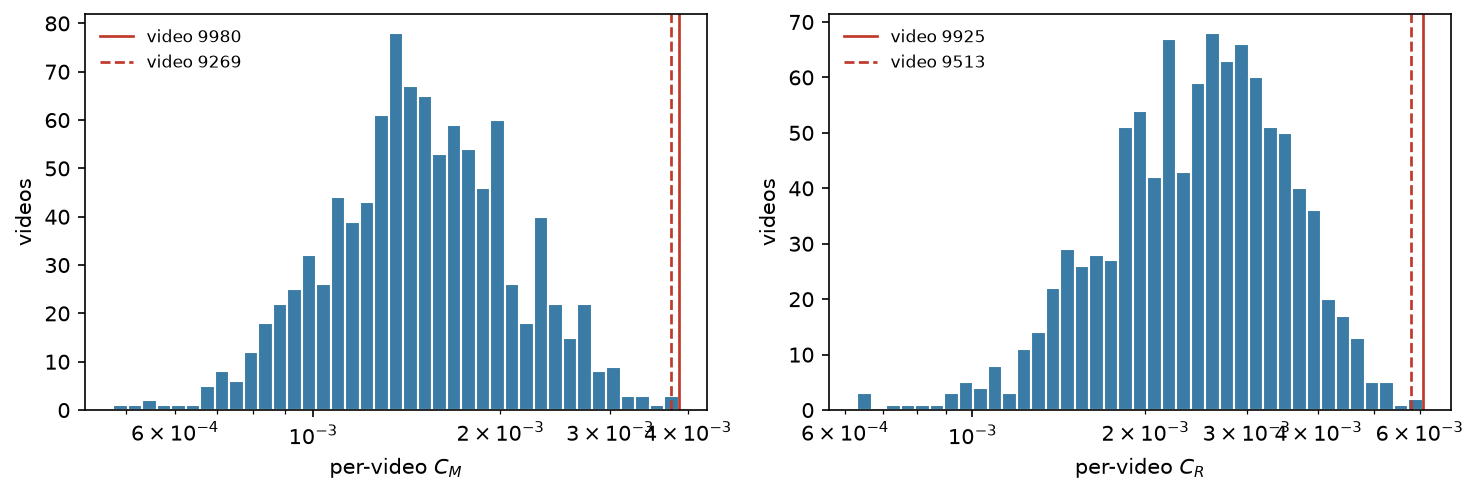
\includegraphics[width=0.9\linewidth]{../Question2/figures/fig4_A_consistency_hist.png}
\caption*{\textbf{Figure 4.} Per-video $C_M$ and $C_R$ of seed-0 model A over the 1,000 test videos (log scale). Red lines: the videos in Figure 3.}
\end{figure}

\paragraph{Q2.6.} Blank ignores the input and Copy-last only repeats it, so both commute with any rearrangement of pixels and have $C_M=C_R=0$, yet their errors (0.0426 and 0.0641) are the worst in Table 3. A small $C_T$ only says that the model treats the transformed clip the same way as the original, not that it treats either one correctly: a model can be consistently wrong. $E_T$ measures correctness on the transformed clip, so the two must be read together.

\paragraph{Q2.7.} Video 9925 under rotation (Figure 3, bottom left). In the rotated clip (row 2) one digit sits at the top and the other at the bottom left, and both drift slowly. Predicting from the rotated input (row 3), the model stretches the top digit downwards into a vertical streak that by $h=3$ reaches the lower digit, so the two digits merge into one column and the top digit becomes unrecognisable. Rotating the original prediction (row 4) instead gives two separate horizontal blobs that stay near their last positions and fade. So on the rotated clip the model invents a downward motion for the top digit that is not in the data and loses it in a smear, while on the upright clip it keeps both digits apart. The motion rule it applies depends on what the digits look like.

\paragraph{Q2.8.} Yes. For model A, $C_R=0.00289$ is about 1.6 times $C_M=0.00176$, and the cost of transforming the clip is larger under rotation ($E_R-E^{(5)}=0.0017$) than under mirroring ($E_M-E^{(5)}=0.0006$). By Q2.1 both transformations give motion that is already common in training, so the motion does not explain the gap. By Q2.2 what differs is appearance: a mirrored digit keeps its upright strokes, while a rotated digit lies on its side and is further from anything in training. The difference therefore comes from appearance.

\begin{table}[H]\centering\small
\caption*{\textbf{Table 4.} Model A at higher speed ($t=1$), mean (seed 0, seed 1). Blank: $E^{(2)}=0.0426$, 0.0425, 0.0426 at $1\times$, $2\times$, $3\times$.}
\begin{adjustbox}{max width=\linewidth}\begin{tabular}{@{}lccccc@{}}
\toprule
 & $E^{(2)}$ $1\times$ & $E^{(2)}$ $2\times$ & $E^{(2)}$ $3\times$ & $E^{(5)}$ $1\times$ & $E^{(5)}$ $2\times$\\
\midrule
A & 0.0189 (0.0193, 0.0184) & 0.0444 (0.0431, 0.0457) & 0.0522 (0.0511, 0.0533) & 0.0222 (0.0227, 0.0216) & 0.0488 (0.0467, 0.0509)\\
Copy-last & 0.0548 & 0.0661 & 0.0703 & 0.0641 & 0.0719\\
\bottomrule
\end{tabular}\end{adjustbox}
\end{table}

\begin{figure}[H]\centering
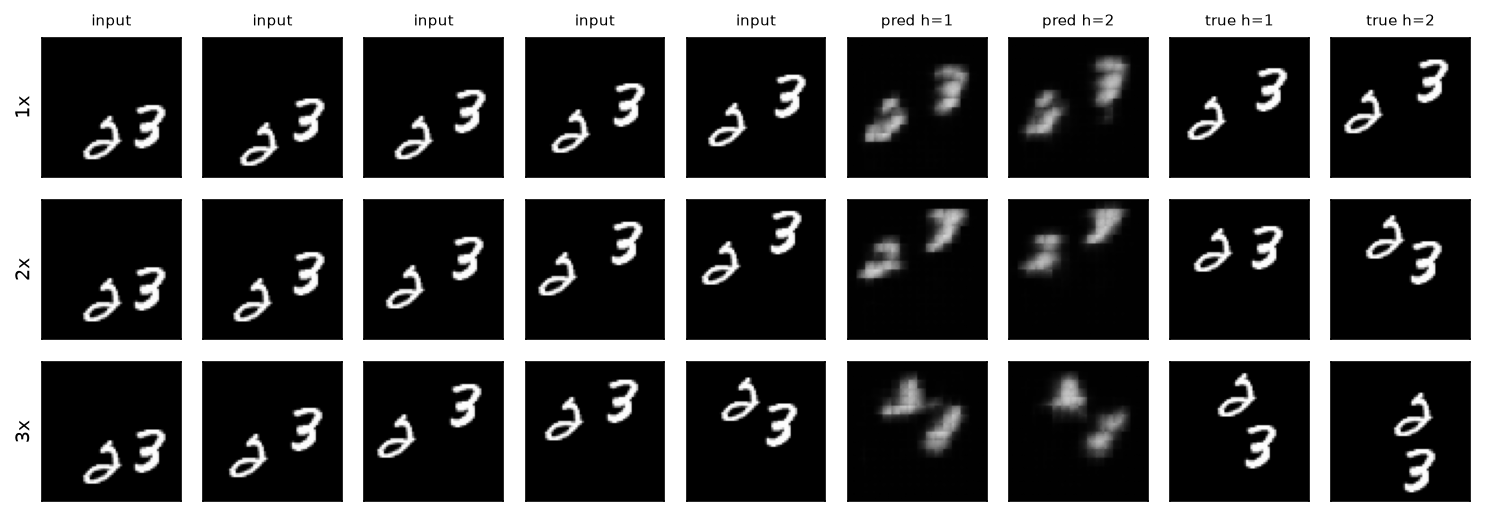
\includegraphics[width=\linewidth]{../Question2/figures/fig5_A_speed.png}
\caption*{\textbf{Figure 5.} Test video 9026 at $1\times$, $2\times$, $3\times$ (seed-0 model A): five input frames, first two predicted and true frames. The digits do not overlap in any displayed true frame.}
\end{figure}

\paragraph{Q2.9.} Model A already falls apart at $2\times$: $E^{(2)}$ rises from 0.0189 to 0.0444, worse than Blank (0.0425), and reaches 0.0522 at $3\times$. This does not agree with the reach estimate, which put $2\times$ (6.6 px/frame) inside the 8 px reach. The estimate missed two things. First, 8 px is the most information can move along the single longest path; to follow a digit the model must also detect its displacement, and in layer~1 the new frame and the previous state meet in one $3\times3$ convolution that spans only one cell (4 px). A 6.6 px jump is not visible there, so the motion has to be both detected and carried forward within the same two-layer budget. Second, the model only learned displacements of about 2--5 px, so even moves within reach are ones it never had to make. In Figure 5, at $1\times$ both digits move correctly but blur. At $2\times$ and $3\times$ the digits stall near their last input position and fade into blobs instead of jumping to the true position. Stalling and fading suggest the model falls back to a blurred copy of the last frame: it does not connect the old and new positions, so it hedges by spreading intensity near where the digit was.

\paragraph{Q2.10.} No. Both explanations predict the same thing here: at $2\times$ and $3\times$ the digits move faster than anything model A saw in training (Figure 1b: 2.1--4.1 px/frame for 80\% of pixels), and at $3\times$ also faster than its 8 px reach. Since model A was trained on $1\times$ only, the two causes are confounded. To separate them, train the same architecture on all three speeds (model C). If the failure is unfamiliar motion, C should recover at $2\times$ and $3\times$. If it is reach, C should improve at $2\times$ (within reach) but still fail at $3\times$, and only a model with larger reach trained on the same speeds (model D) should fix $3\times$.

% ---------------------------------------------------------------------
\subsection*{4. What Can Data Fix?}

\paragraph{Q2.11 (written before training B--D).} Model B (symmetry augmentation) will close most of the mirror and rotation gap (lower $C_M$, $C_R$ and $E_M$, $E_R$ close to $E^{(5)}$ at $1\times$) but leave the $2\times$ and $3\times$ failure unchanged. Model C (speed augmentation) will fix $2\times$ and improve $3\times$ without fully fixing it, because 10 px/frame is still beyond its 8 px reach. Model D (larger reach, speed augmentation) will fix $3\times$ as well, and neither C nor D will fix mirror or rotation.

\begin{table}[H]\centering\small
\caption*{\textbf{Table 5.} Models A--D on the test split, mean (seed 0, seed 1). Hardware: MacBook Pro (2021), Apple M1 Pro, 32 GB, PyTorch \texttt{mps}. Training time is per epoch; inference is all 1,000 test videos ($1\times$, $t=1$, batch 32).}
\begin{adjustbox}{max width=\linewidth}\begin{tabular}{@{}lcccc@{}}
\toprule
 & A & B & C & D\\
\midrule
$E^{(5)}$ $1\times$ & 0.0222 (0.0227, 0.0216) & 0.0228 (0.0235, 0.0221) & 0.0279 (0.0276, 0.0283) & 0.0275 (0.0279, 0.0272)\\
$C_M$ & 0.00176 (0.00158, 0.00195) & 0.00121 (0.00125, 0.00117) & 7.94e-4 (7.99e-4, 7.89e-4) & 8.35e-4 (9.69e-4, 7.00e-4)\\
$E_M$ & 0.0228 (0.0233, 0.0223) & 0.0228 (0.0235, 0.0221) & 0.0282 (0.0278, 0.0285) & 0.0277 (0.0280, 0.0274)\\
$C_R$ & 0.00289 (0.00260, 0.00318) & 0.00141 (0.00156, 0.00126) & 0.00198 (0.00173, 0.00223) & 0.00192 (0.00171, 0.00213)\\
$E_R$ & 0.0239 (0.0242, 0.0236) & 0.0227 (0.0233, 0.0220) & 0.0291 (0.0287, 0.0295) & 0.0286 (0.0287, 0.0284)\\
$E^{(2)}$ $1\times$ & 0.0189 (0.0193, 0.0184) & 0.0191 (0.0198, 0.0183) & 0.0241 (0.0239, 0.0243) & 0.0247 (0.0248, 0.0246)\\
$E^{(2)}$ $2\times$ & 0.0444 (0.0431, 0.0457) & 0.0441 (0.0439, 0.0444) & 0.0295 (0.0295, 0.0295) & 0.0292 (0.0296, 0.0289)\\
$E^{(2)}$ $3\times$ & 0.0522 (0.0511, 0.0533) & 0.0513 (0.0515, 0.0511) & 0.0339 (0.0338, 0.0340) & 0.0327 (0.0328, 0.0326)\\
Parameters & 480,784 & 480,784 & 480,784 & 480,784\\
Train (s/epoch) & 25.6 (24.8, 26.4) & 24.0 (24.2, 23.9) & 23.7 (23.6, 23.8) & 27.9 (28.0, 27.7)\\
Inference (s) & 0.721 (0.728, 0.713) & 0.714 (0.711, 0.716) & 0.711 (0.710, 0.711) & 0.920 (0.924, 0.917)\\
\bottomrule
\end{tabular}\end{adjustbox}
\end{table}

\begin{figure}[H]\centering
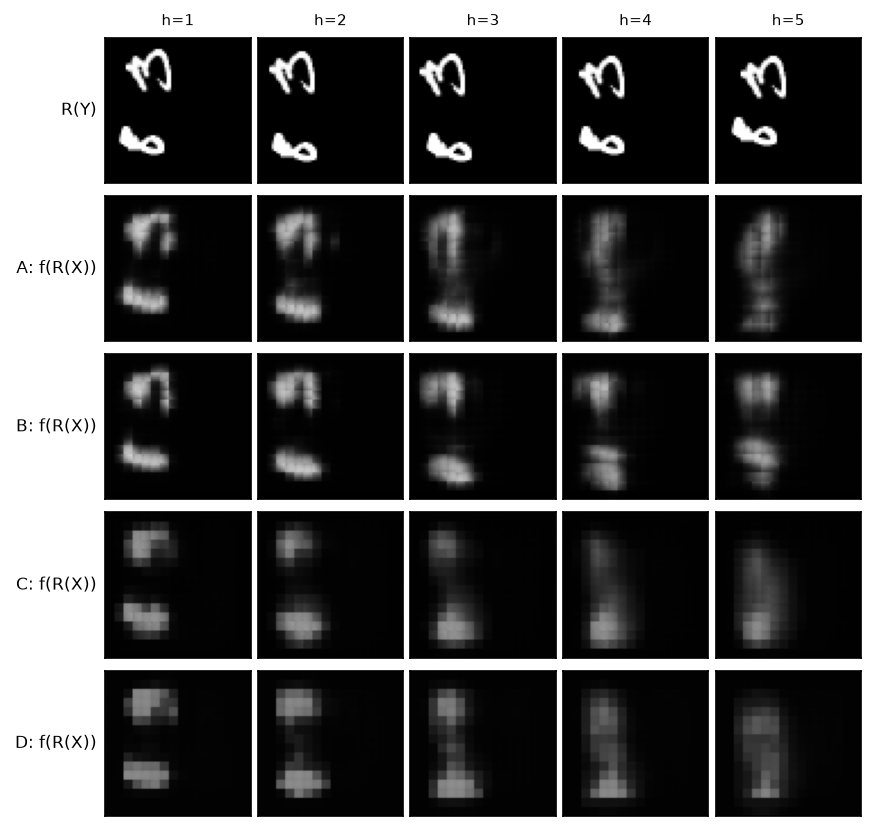
\includegraphics[width=0.48\linewidth]{../Question2/figures/figS_rotation_video9925.png}\hfill
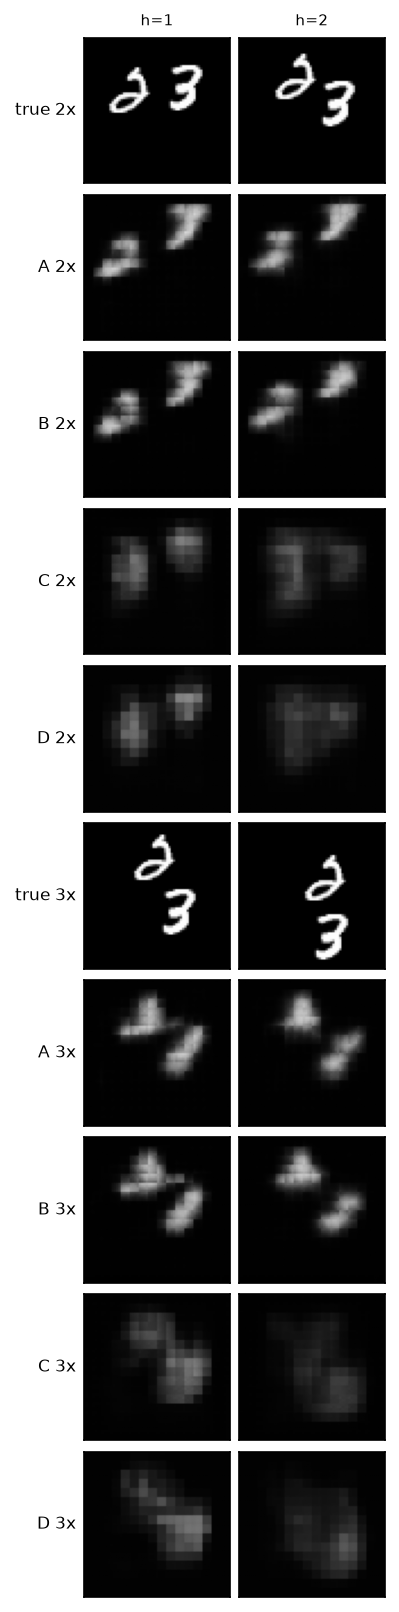
\includegraphics[width=0.17\linewidth]{../Question2/figures/figS_speed_video9026.png}
\caption*{\textbf{Figure S1.} The same clips under models A--D (seed 0). Left: video 9925 rotated, truth $R(Y)$ and $f(R(X))$ for each model. Right: video 9026, first two horizons at $2\times$ and $3\times$.}
\end{figure}

\paragraph{Q2.12.} Model D is model A with a dilation of 2 in the layer-2 convolution; everything else (patch 4, 64 channels, $3\times3$ kernels, rollout, training) is unchanged, and dilation adds no weights, so it has 480,784 parameters. Using the conventions of Q2.3: layer~1 moves information by at most 1 cell and layer~2, now spanning $\pm2$ cells, by at most 2. The longest path in one step, $u_\tau$ or $h^{(1)}_{\tau-1}\to$ layer~1 $\to$ layer~2 $\to\hat x_{\tau+1}$, therefore covers $1+2=3$ cells $=$ \textbf{12 px}, strictly larger than model A's 8 px. Offsets $\{-1,0,1\}+\{-2,0,2\}$ cover every cell in $-3\ldots3$, so no shift within the reach is missing (dilation 2 in both layers would reach only even offsets). Three candidates were trained with seed~0 under model D's protocol and compared on the validation split (\texttt{results/d\_selection.json}): dilations (1,~2) at 12 px, (1,~3) at 16 px, and $5\times5$ kernels with 46 channels at 16 px (709,520 parameters). Mean validation $E^{(2)}$ over the three speeds was 0.0287, 0.0307 and 0.0395, and the $5\times5$ model never left the blank solution, so (1,~2) was chosen and its seed-0 run is model D's seed~0.

\paragraph{Q2.13.} \emph{Rotation (and mirror) gap: appearance.} B changes only the training orientations, halves $C_R$ (0.00289 to 0.00141) and lowers $C_M$ by about a third (0.00176 to 0.00121); $E_R$ falls from 0.0239 to 0.0227, level with its $E^{(5)}$ of 0.0228, while its speed errors are unchanged (0.0441, 0.0513). \emph{Failure at $2\times$: unfamiliar motion.} C changes only the training speeds and cuts $E^{(2)}$ at $2\times$ from 0.0444 to 0.0295, without any extra reach. \emph{Failure at $3\times$: mostly unfamiliar motion, with a small reach part.} C cuts it from 0.0522 to 0.0339; D, which adds only reach, lowers it further to 0.0327, about 3.5\% (lower in both seeds: 0.0328 against 0.0338, 0.0326 against 0.0340). C did not ``still do badly'' at $3\times$: although 10 px exceeds its 8 px one-step reach, the recurrent state can carry a velocity estimate over two steps (16 px), which is why speed training alone helps. Reach still matters as a hard limit: within one update a pixel can only affect outputs within the reach, and data can change the weights but cannot create a connection that the computation does not have. Figure S1 adds a caution: at $2\times$ and $3\times$ C and D lower the error partly by spreading intensity over the likely positions rather than tracking the digits sharply.

\paragraph{Q2.14.} Yes. Speed augmentation costs accuracy at $1\times$: $E^{(5)}$ rises from 0.0222 (A) to 0.0279 (C) and 0.0275 (D), about 25\%, and the predictions are blurrier (Figure S1). The same 480,784 parameters and 30 epochs now cover three speed regimes. Symmetry augmentation costs almost nothing (B: 0.0228). The trade is worth it if the forecaster must face unknown speeds: for D, the $3\times$ error falls by 37\% and the $2\times$ error by 34\% relative to A. If only $1\times$ clips matter, model A remains the most accurate.

% ---------------------------------------------------------------------
\subsection*{5. The Final Model}

\paragraph{Exact consistency.} For any $h\in G$, substitute $g'=gh$, which runs over all of $G$ as $g$ does, so $g=g'h^{-1}$ and $g^{-1}=h\,g'^{-1}$:
\[
\bar f(hX)=\frac18\sum_{g\in G} g^{-1}f(ghX)=\frac18\sum_{g'\in G} h\,g'^{-1}f(g'X)=h\,\bar f(X),
\]
since $h$ is a linear rearrangement of pixels and commutes with the average. With $h=M$ and $h=R$, $\bar f(T(X))=T(\bar f(X))$, so $C_M=C_R=0$ for any $f$. Table~6 confirms this to about $10^{-16}$.

\paragraph{Choice of final model.} Symmetrised D. Table~5 suggested D+B might help: B halved $C_R$ at no cost on $1\times$ clips, and a base model whose eight views agree more could give a sharper average. D+B was therefore trained (both seeds) and compared with D, both symmetrised, on the validation split only, using the same criterion as for model D (mean $E^{(2)}$ over $1\times$, $2\times$, $3\times$, averaged over seeds; \texttt{results/final\_selection.json}). Symmetrised D scored 0.0286 and symmetrised D+B 0.0288, with D equal or slightly better at every speed, so D was kept. Once the forecaster is symmetrised, symmetry augmentation adds nothing measurable.

\begin{table}[H]\centering\small
\caption*{\textbf{Table 6.} Symmetrised models, mean (seed 0, seed 1). Training time is that of the underlying model; inference includes all eight transformations, forward passes, inverses and the averaging.}
\begin{adjustbox}{max width=\linewidth}\begin{tabular}{@{}lcc@{}}
\toprule
 & Symmetrised B & Symmetrised D (final)\\
\midrule
$E^{(5)}$ $1\times$ & 0.0221 (0.0228, 0.0215) & 0.0275 (0.0278, 0.0272)\\
$C_M$ & 8.11e-17 (8.75e-17, 7.46e-17) & 5.67e-17 (5.08e-17, 6.25e-17)\\
$E_M$ & 0.0221 (0.0228, 0.0215) & 0.0275 (0.0278, 0.0272)\\
$C_R$ & 6.57e-17 (7.14e-17, 6.00e-17) & 4.40e-17 (3.96e-17, 4.84e-17)\\
$E_R$ & 0.0221 (0.0228, 0.0215) & 0.0275 (0.0278, 0.0272)\\
$E^{(2)}$ $1\times$ & 0.0186 (0.0194, 0.0179) & 0.0247 (0.0248, 0.0246)\\
$E^{(2)}$ $2\times$ & 0.0434 (0.0432, 0.0436) & 0.0293 (0.0296, 0.0289)\\
$E^{(2)}$ $3\times$ & 0.0503 (0.0505, 0.0501) & 0.0327 (0.0327, 0.0326)\\
Parameters & 480,784 & 480,784\\
Train (s/epoch) & 24.0 (24.2, 23.9) & 27.9 (28.0, 27.7)\\
Inference (s) & 5.03 (5.03, 5.03) & 6.51 (6.51, 6.50)\\
\bottomrule
\end{tabular}\end{adjustbox}
\end{table}

\begin{figure}[H]\centering
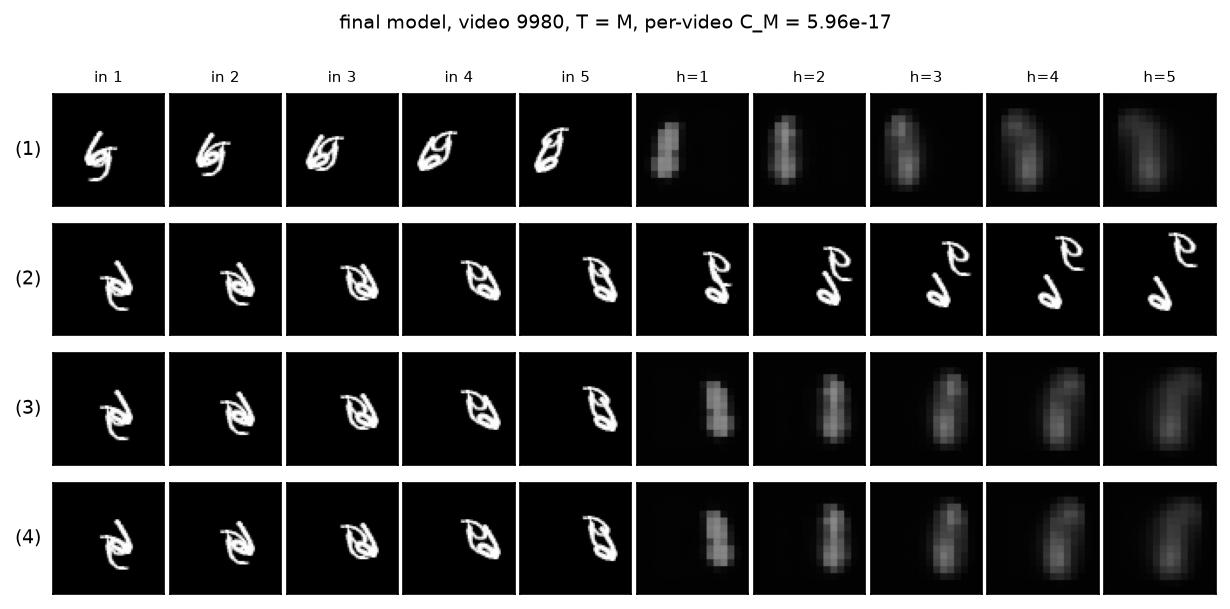
\includegraphics[width=0.49\linewidth]{../Question2/figures/fig6a_final_M1_video9980.png}\hfill
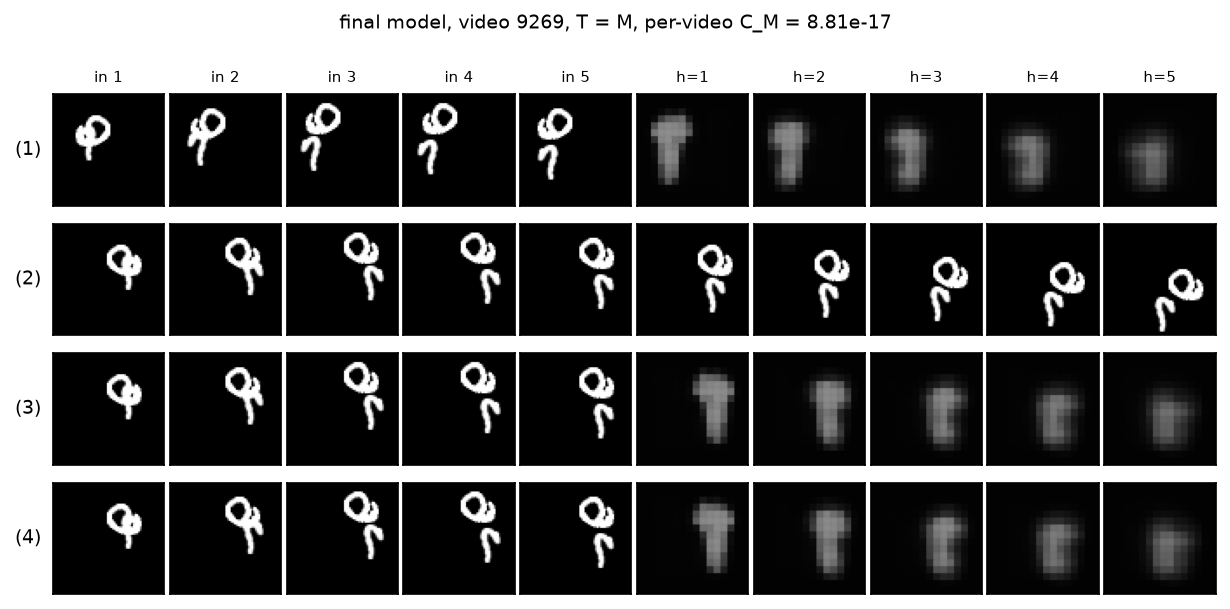
\includegraphics[width=0.49\linewidth]{../Question2/figures/fig6a_final_M2_video9269.png}\\[4pt]
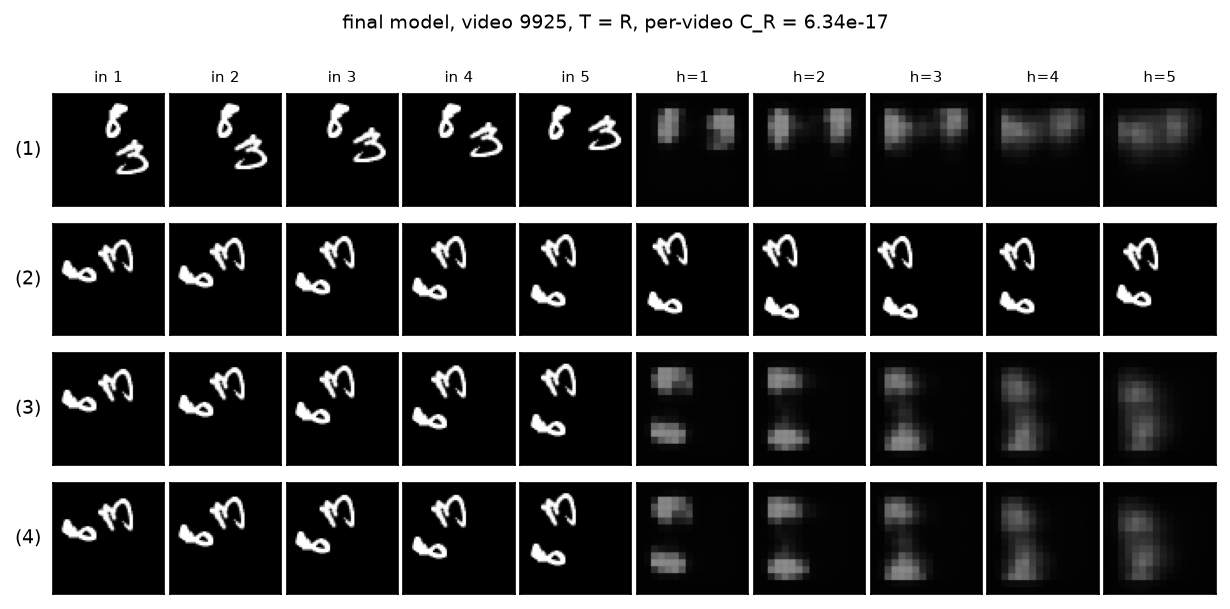
\includegraphics[width=0.49\linewidth]{../Question2/figures/fig6a_final_R1_video9925.png}\hfill
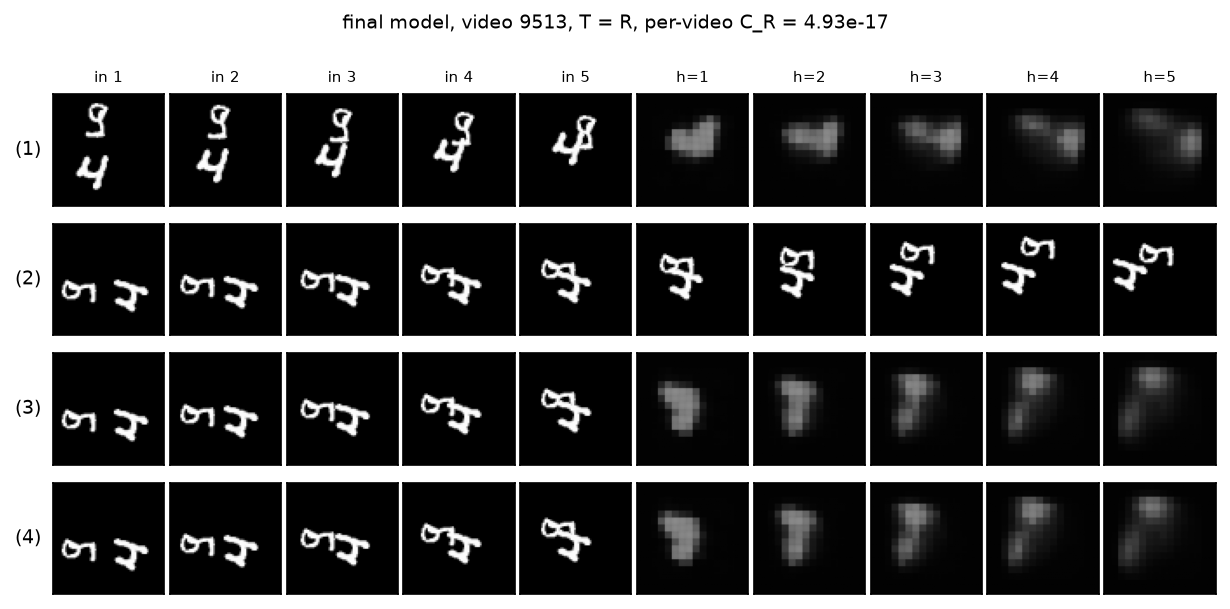
\includegraphics[width=0.49\linewidth]{../Question2/figures/fig6a_final_R2_video9513.png}\\[6pt]
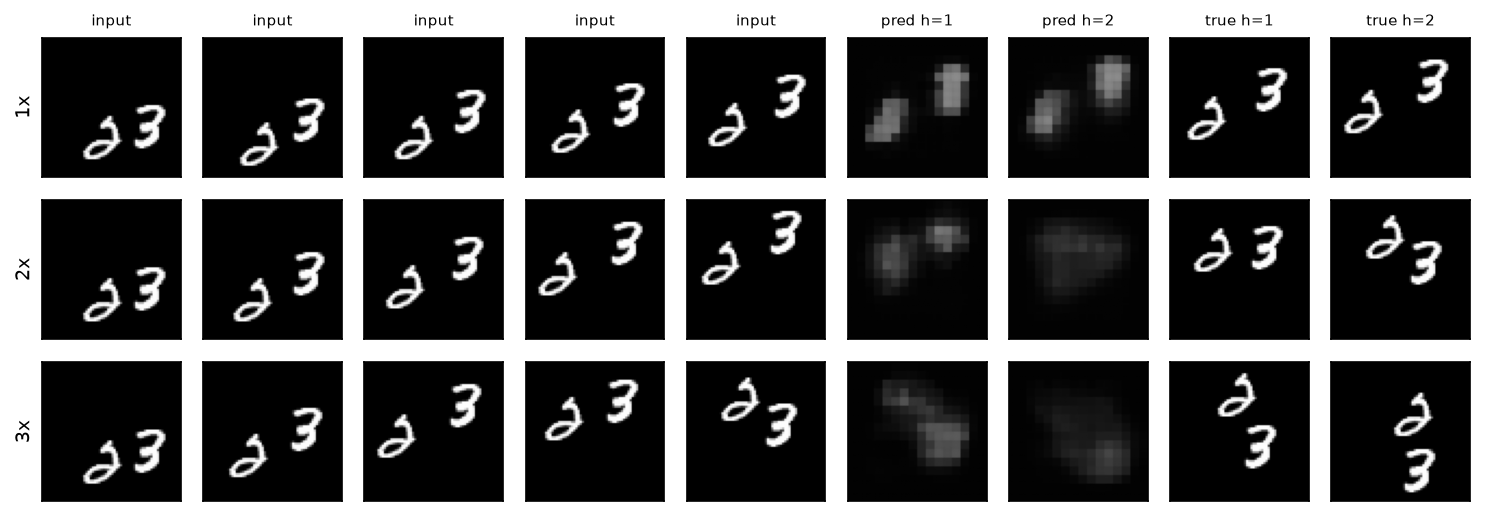
\includegraphics[width=\linewidth]{../Question2/figures/fig6b_final_speed.png}
\caption*{\textbf{Figure 6.} Final model (symmetrised D, seed 0). (a) Top four panels: the videos and rows of Figure 3. GIFs: \texttt{Question2/gifs/fig6a\_final\_M\_video9980.gif}, \texttt{fig6a\_final\_M\_video9269.gif}, \texttt{fig6a\_final\_R\_video9925.gif}, \texttt{fig6a\_final\_R\_video9513.gif}. (b) Bottom: video 9026 at $1\times$, $2\times$, $3\times$ as in Figure 5.}
\end{figure}

\paragraph{Q2.15.} Learned symmetry (B) lowers the gaps ($C_M=0.00121$, $C_R=0.00141$) but does not remove them; the loss only encourages consistency on the training clips. Built-in symmetry is exact ($C_M,C_R\approx10^{-16}$) because, by the argument above, it holds for any weights. Accuracy on the original clips is not hurt: symmetrised B has $E^{(5)}=0.0221$ against 0.0228 for B, and symmetrised D matches D (0.0275); on transformed clips $E_M=E_R=E^{(5)}$ by construction. The cost is inference: eight forward passes make it about seven times slower (0.714 to 5.03 s for B, 0.920 to 6.51 s for D). Averaging blurs when the eight views disagree, so built-in symmetry should hurt most when the base model is far from consistent or when the task itself is not symmetric. Here the views already agreed closely, and since squared error is convex, the average is never worse than the average error of the eight views; so it did not hurt on the numbers, although Figure 6 is visibly softer than Figure 3. Making the views agree more before averaging did not sharpen the result either: symmetrised D+B was no better than symmetrised D on validation.

\paragraph{Q2.16.} Partly. For video 9925, rows 3 and 4 of Figure 6(a) are now identical ($C_R=6.34\times10^{-17}$): symmetrisation removed the downward streak that model A invented only for the rotated clip, so the motion rule no longer depends on orientation. The prediction is still not right: both digits are coarse blobs that stay near their last positions and by $h=4$--5 smear into one column, while in the truth they stay apart. Symmetrisation fixed the consistency; speed training and the larger reach do not help this slow clip and add blur.

\paragraph{Q2.17 Final verdict.} Yes, the model did partly learn motion, but it cannot be said that it has fully learned how things move. It applies the same rule in all eight orientations exactly, and with speed training its $2\times$ and $3\times$ errors are about a third lower than model A's, so its predictions depend on motion and not only on how the training clips look. However, lower error is not proof of tracking. Convincing evidence would be predicted digit centres following the true trajectories, including bounces, at every speed and orientation, and sensible predictions at untrained speeds like $1.5\times$ or $4\times$. That evidence is missing: predictions blur within two or three steps, digits lose their identity, and on fast clips (Figure 6b) part of the gain comes from spreading intensity over likely positions. One test it still fails is keeping two overlapping digits apart after they separate (video 9000).
